\chapter{Mass Spectrometry and Atomic Spectroscopy}\label{ch:b2:mass-spec-atomic}

Fireworks are red with strontium salts, green with barium salts, yellow with sodium: a flame turns
atoms into light of colours that identify them. A mass spectrometer, more modestly in appearance,
weighs single molecules, sorts them by their isotopes and breaks them into pieces whose masses tell
how they were built. Both techniques answer the question ``what is in this sample, and how much?''
from very small amounts, the first for molecules, the second for elements.

\begin{omfigure}
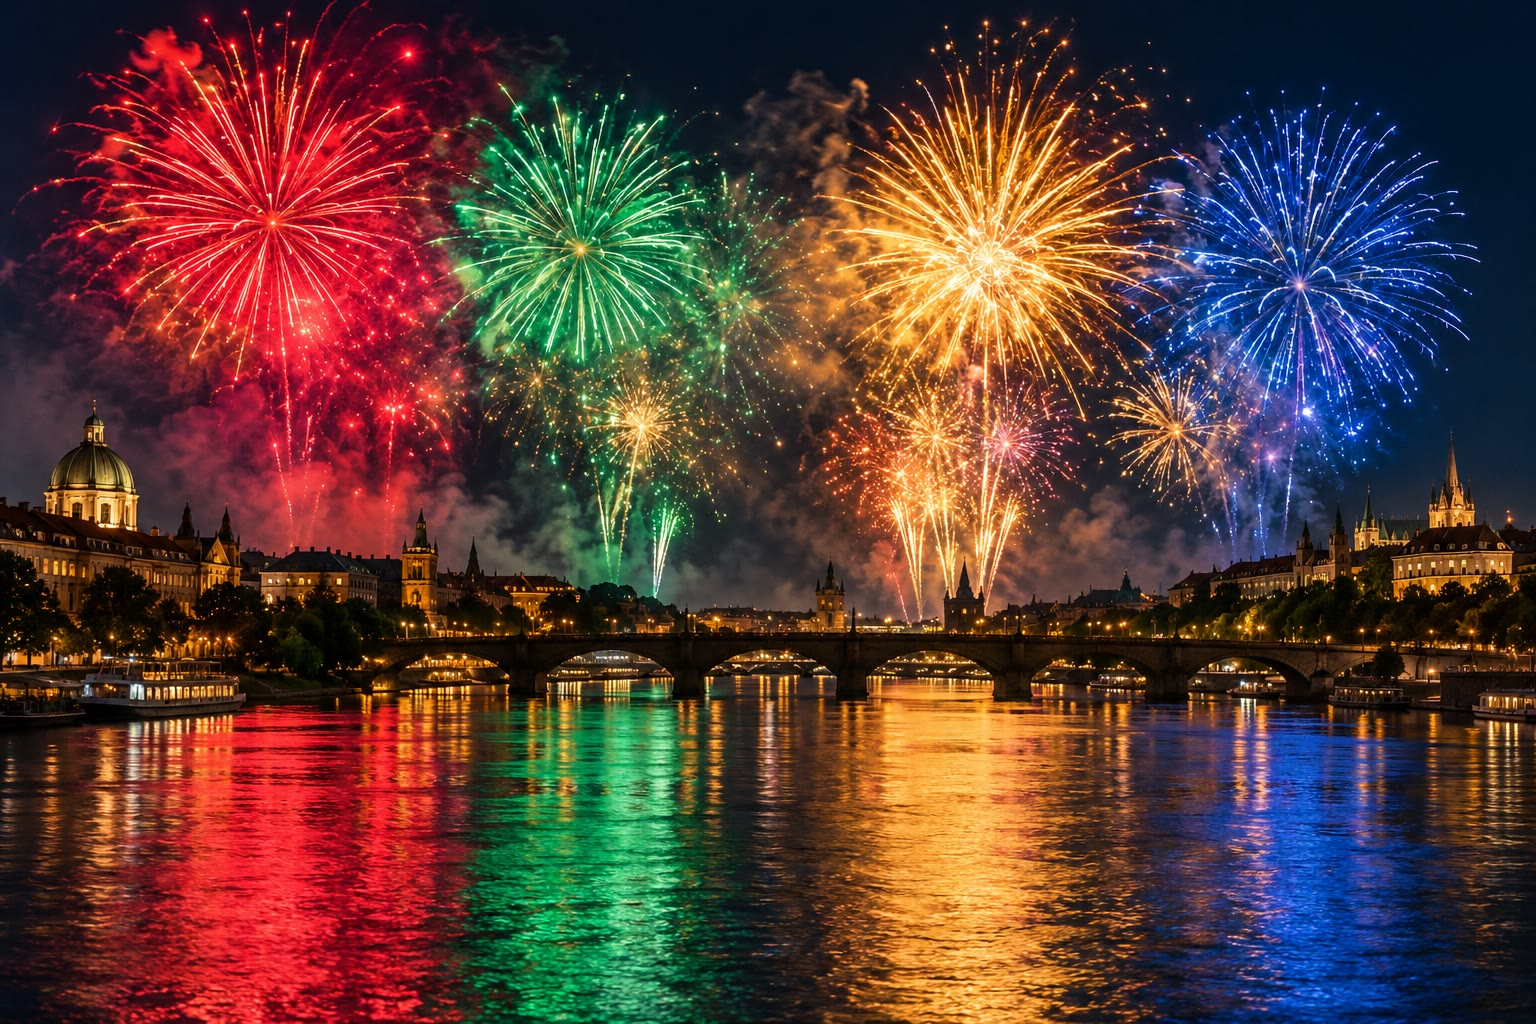
\includegraphics[width=0.58\linewidth]{images/book3/ai/b2-32-fireworks.jpg}

{\small Fireworks over a river (illustration). The yellow of sodium is the light of its atoms; the
deep reds and greens come largely from small molecules of strontium and barium formed in the flame.}
\end{omfigure}

\begin{recall}
The school volume: isotopes and their abundances. The Year 1 volume: energy levels and spectral
lines, absorbance and the Beer--Lambert law, carbocations and radicals, the degree of unsaturation.
\Cref{ch:b2:chromatography}: \omterm{def:b2:chromatography:techniques}{gas chromatography}, which often feeds a mass spectrometer.
\end{recall}

\section{The mass spectrometer}

\begin{definition}[Mass spectrometry]\label{def:b2:mass-spec-atomic:spectrum}
\emph{Mass spectrometry}\index{mass spectrometry} turns the molecules of a sample into gaseous ions,
separates the ions according to their \emph{mass-to-charge ratio}\index{mass-to-charge ratio} $m/z$
(the mass in unified atomic mass units divided by the number of charges) and counts them. The
\emph{mass spectrum}\index{mass spectrum} plots the abundance of the ions against $m/z$, usually as
relative intensities; its most intense peak, set to 100, is the \emph{base peak}\index{base peak}.
\end{definition}

A spectrometer has three parts. The source makes ions. In electron ionisation (EI) the vapour of the
sample crosses a beam of electrons of \qty{70}{eV}, which knock an electron out of the molecules and
leave them with excess energy, so that many break apart. In electrospray ionisation (ESI) a solution is
sprayed from a charged needle; as the droplets evaporate, molecules leave them carrying an extra proton
(or a sodium ion), intact: the method of choice for large, fragile molecules. The analyser then sorts
the ions, and a detector counts them.

\begin{omfigure}
\begin{tikzpicture}[x=1cm, y=1cm]
\draw[black!70, fill=omDef!10, rounded corners=2pt] (0,-0.6) rectangle (1.6,0.6);
\node[font=\small, align=center] at (0.8,0) {ion\\source};
\draw[black!70] (2.0,-0.7) -- (2.0,0.7); \draw[black!70] (2.4,-0.7) -- (2.4,0.7);
\node[font=\footnotesize] at (2.2,1.0) {grids, $U$};
\draw[black!70] (2.6,-0.5) rectangle (8.4,0.5);
\node[font=\small] at (5.6,0.8) {field-free drift tube, length $L$};
\draw[black!70, fill=black!15] (8.5,-0.6) rectangle (8.8,0.6);
\node[font=\small, align=center] at (9.6,0) {detector};
\foreach \x/\c in {3.4/omThm, 4.6/omDef, 6.3/omMeth}{\fill[\c] (\x,0) circle (0.1);}
\draw[->, thick] (6.6,0) -- (7.4,0);
\node[font=\footnotesize, align=center] at (5.5,-0.85) {light ions fly ahead, heavy ones lag};
\end{tikzpicture}
\par\vspace{4pt}

{\small A time-of-flight analyser (schematic). Ions accelerated through the same potential difference
$U$ leave with the same kinetic energy; in the drift tube the lighter ones travel faster and reach the
detector first.}
\end{omfigure}

\begin{proposition}[Time of flight]\label{prop:b2:mass-spec-atomic:time-of-flight}
An ion of mass $m$ and charge $ze$, accelerated from rest through a potential difference $U$, crosses a
field-free tube of length $L$ in
\begin{equation*}
t = L\sqrt{\frac{m}{2zeU}}:
\end{equation*}
the flight time grows as the square root of $m/z$.
\end{proposition}

\begin{proof}
Energy conservation in the accelerating field gives $\tfrac12mv^2 = zeU$, so $v = \sqrt{2zeU/m}$, and
the tube is crossed at constant speed: $t = L/v$.
\end{proof}

Other analysers sort ions differently: a quadrupole lets through only the ions of one $m/z$ at a time,
selected by oscillating voltages on four rods; a magnetic sector bends the ions on circles whose radius
depends on their momentum. In all of them only $m/z$ is measured; most ions made by EI carry one
charge, so $m/z$ is simply their mass.

\section{The molecular ion}

\begin{definition}[Molecular and fragment ions]\label{def:b2:mass-spec-atomic:molecular-ion}
The \emph{molecular ion}\index{molecular ion} $\mathrm M^{+\bullet}$ is the radical cation formed when a
molecule loses one electron; its $m/z$ is the molar mass of the molecule made of the most abundant
isotopes. A \emph{fragment ion}\index{fragment ion} comes from the molecular ion by the breaking of
bonds.
\end{definition}

The \omterm{def:b2:mass-spec-atomic:molecular-ion}{molecular ion} gives the molecular mass, the first fact about an unknown. It is sometimes weak or
absent in EI, when the \omterm{def:b2:mass-spec-atomic:molecular-ion}{molecular ion} breaks too easily; electrospray, which gives $[\mathrm M +
\mathrm H]^+$ at one unit above, then confirms it.

\begin{definition}[Nitrogen rule]\label{def:b2:mass-spec-atomic:nitrogen-rule}
The \emph{nitrogen rule}\index{nitrogen rule} states that a molecule has an odd nominal mass (the sum
of the mass numbers of its most abundant isotopes) if and only if it contains an odd number of nitrogen
atoms.
\end{definition}

\begin{proposition}[Validity of the nitrogen rule]\label{prop:b2:mass-spec-atomic:nitrogen-rule}
The \omterm{def:b2:mass-spec-atomic:nitrogen-rule}{nitrogen rule} holds for every molecule without unpaired electrons built from C, H, N, O, S and the
halogens.
\end{proposition}

\begin{proof}
The nominal masses are even for C (12), N (14), O (16) and S (32), odd for H (1) and the halogens (19,
35, 79, 127). The valences are even for C, O and S, odd for H, N and the halogens. In a molecule
without unpaired electrons, every bond uses one valence of each of its two atoms, so the sum of all
valences is even, and the number of atoms of odd valence, $n_{\ce{H}} + n_{\ce{X}} + n_{\ce{N}}$, is
even. The parity of the nominal mass is that of $n_{\ce{H}} + n_{\ce{X}}$, which is therefore that of
$n_{\ce{N}}$.
\end{proof}

\begin{definition}[Isotope pattern]\label{def:b2:mass-spec-atomic:isotope-pattern}
The \emph{isotope pattern}\index{isotope pattern} of an ion is the group of peaks at $M$, $M+1$,
$M+2$, \dots\ produced by the molecules containing heavier isotopes, with intensities in proportion to
the abundances of those isotopic forms.
\end{definition}

\begin{proposition}[The $M+1$ peak]\label{prop:b2:mass-spec-atomic:m-plus-one}
For an ion with $n_C$ carbon atoms and no other element with a significant $+1$ isotope,
\begin{equation*}
\frac{I(M+1)}{I(M)} \approx n_C\,\frac{a_{13}}{a_{12}} \approx n_C \times 1.1~\%,
\end{equation*}
where $a_{12} = 0.989$ and $a_{13} = 0.011$ are the amount fractions of the two carbon isotopes.
% ledger: iso:C12, iso:C13
\end{proposition}

\begin{proof}
The probability that all $n_C$ carbons are \ce{^{12}C} is $a_{12}^{n_C}$; that exactly one is
\ce{^{13}C} is $n_C\,a_{13}a_{12}^{n_C - 1}$ (binomial law). The ratio is $n_C\,a_{13}/a_{12}$, and the
other contributions (two \ce{^{13}C}, \ce{^2H}, \ce{^{15}N}) are smaller by a factor of the order of
$a_{13}$ or below.
\end{proof}

\begin{proposition}[Chlorine and bromine]\label{prop:b2:mass-spec-atomic:halogen-patterns}
For an ion with $p$ chlorine and $q$ bromine atoms, the intensities of $M$, $M+2$, $M+4$, \dots\ are
the coefficients of the expansion of $(a_{35} + a_{37}x)^p(a_{79} + a_{81}x)^q$ in powers of $x$, each
power of $x$ standing for 2 mass units. With $a_{35} = 0.758$, $a_{37} = 0.242$, $a_{79} = 0.5069$ and
$a_{81} = 0.4931$, one chlorine gives $M : M+2 \approx 3 : 1$ and one bromine $\approx 1 : 1$.
% ledger: iso:Cl35, iso:Cl37, iso:Br79, iso:Br81
\end{proposition}

\begin{proof}
Each halogen atom independently is the light isotope or the heavy one, which adds 2 to the mass. The
probability of a given number $j$ of heavy atoms is the coefficient of $x^j$ in the product of one factor
per atom, which is the expansion stated (the binomial law, per element).
\end{proof}

\begin{omfigure}
\pgfplotsset{clu/.style={width=0.25\linewidth, height=3.3cm, ybar, bar width=5pt, ymin=0, ymax=118,
  xmin=-1.2, xmax=5.2, xtick={0,2,4}, xticklabels={$M$,$M\!+\!2$,$M\!+\!4$},
  tick label style={font=\tiny}, ytick=\empty, axis x line=bottom, axis y line=none,
  title style={font=\small, yshift=-4pt}, nodes near coords, nodes near coords style={font=\tiny},
  point meta=y, every node near coord/.append style={/pgf/number format/fixed, /pgf/number format/precision=0}}}
\begin{tikzpicture}
\begin{axis}[clu, title={Cl}]
\addplot[fill=omDef!55, draw=omDef, y filter/.expression={y==0 ? nan : y}] table[x=off, y=Cl] {figdata/out/bachelor-2-mass-spectra-a.dat};
\end{axis}
\end{tikzpicture}\hfill
\begin{tikzpicture}
\begin{axis}[clu, title={Cl$_2$}]
\addplot[fill=omDef!55, draw=omDef] table[x=off, y=Cl2] {figdata/out/bachelor-2-mass-spectra-a.dat};
\end{axis}
\end{tikzpicture}\hfill
\begin{tikzpicture}
\begin{axis}[clu, title={Br}]
\addplot[fill=omThm!45, draw=omThm, y filter/.expression={y==0 ? nan : y}] table[x=off, y=Br] {figdata/out/bachelor-2-mass-spectra-a.dat};
\end{axis}
\end{tikzpicture}\hfill
\begin{tikzpicture}
\begin{axis}[clu, title={Br$_2$}]
\addplot[fill=omThm!45, draw=omThm] table[x=off, y=Br2] {figdata/out/bachelor-2-mass-spectra-a.dat};
\end{axis}
\end{tikzpicture}\hfill
\begin{tikzpicture}
\begin{axis}[clu, title={ClBr}]
\addplot[fill=omMeth!45, draw=omMeth] table[x=off, y=ClBr] {figdata/out/bachelor-2-mass-spectra-a.dat};
\end{axis}
\end{tikzpicture}

{\small \omterm{def:b2:mass-spec-atomic:isotope-pattern}{Isotope patterns} of ions containing chlorine and bromine, computed from the isotopic
abundances (\cref{prop:b2:mass-spec-atomic:halogen-patterns}); the most intense peak of each group is
set to 100. The patterns are fingerprints: 3 : 1 for one chlorine, 1 : 1 for one bromine, 1 : 2 : 1
for two bromines.}
% figdata: bachelor-2/mass-spectra.py part a
\end{omfigure}

\begin{definition}[Exact mass]\label{def:b2:mass-spec-atomic:exact-mass}
The \emph{monoisotopic mass}\index{monoisotopic mass} of an ion is the sum of the exact masses of its
most abundant isotopes (\ce{^{12}C} = 12 exactly, \ce{^1H} = 1.007825, \ce{^{16}O} = 15.994915,
\ce{^{14}N} = 14.003074 u). \emph{High-resolution mass spectrometry}\index{high-resolution mass
spectrometry} measures $m/z$ to a few thousandths of a unit or better, enough to tell ions of the same
nominal mass but different formulas apart.
% ledger: mass:C12, mass:H1, mass:O16, mass:N14
\end{definition}

\begin{proposition}[Resolving power]\label{prop:b2:mass-spec-atomic:resolving}
Two ions of masses $m$ and $m + \Delta m$ are separated by an analyser of resolving power at least
$R = m/\Delta m$. At nominal mass 28, separating \ce{CO+} (27.9949) from \ce{N2+} (28.0061) needs $R
\approx 2.5 \times 10^3$; separating \ce{N2+} from \ce{C2H4+} (28.0313), $R \approx 1.1 \times 10^3$.
\end{proposition}

\begin{proof}
The resolving power is defined as $m/\Delta m$ for the smallest $\Delta m$ the analyser separates. The
exact masses follow from the isotopic masses: $12 + 15.994915$, $2 \times 14.003074$, $24 + 4 \times
1.007825$; then $28/(28.0061 - 27.9949) \approx 2.5 \times 10^3$ and $28/(28.0313 - 28.0061) \approx
1.1 \times 10^3$.
\end{proof}

\section{Fragmentation}

The \omterm{def:b2:mass-spec-atomic:molecular-ion}{molecular ion} made by EI carries far more energy than any bond needs to break, and it breaks along
the paths that give the most stable products: stabilised cations, small stable neutral molecules or
radicals. The fragments are read as losses from $M$ (15 for \ce{CH3}, 29 for \ce{C2H5} or \ce{CHO}, 18
for water, 28 for CO or ethene) and as characteristic ions.

\begin{definition}[Two fragmentations]\label{def:b2:mass-spec-atomic:fragmentation}
In an \emph{$\alpha$-cleavage}\index{alpha-cleavage@$\alpha$-cleavage}, a bond to the carbon next to a
heteroatom or a carbonyl breaks, leaving a cation stabilised by the heteroatom's lone pair (an \omterm{def:b2:aromatic-substitution:friedel-crafts}{acylium
ion} $\mathrm{R{-}C{\equiv}O^+}$ for a ketone, an iminium ion for an amine). The \emph{McLafferty
rearrangement}\index{McLafferty rearrangement} of a carbonyl compound transfers a hydrogen from the
$\gamma$ carbon to the carbonyl oxygen and breaks the $\alpha$--$\beta$ bond, releasing an alkene and an
\omterm{def:b2:enolates-aldol:tautomerism}{enol} radical cation.
\end{definition}

\begin{omfigure}
\begin{tikzpicture}
\begin{axis}[width=0.48\linewidth, height=4.6cm, xmin=10, xmax=80, ymin=0, ymax=118,
  xlabel={$m/z$}, ylabel={relative intensity}, label style={font=\small}, tick label style={font=\scriptsize},
  title={\small butan-2-one}, ycomb, xtick={15,29,43,57,72}]
\addplot[omDef, thick] table[x=mz, y=I] {figdata/out/bachelor-2-mass-spectra-b.dat};
\node[font=\tiny, anchor=south] at (axis cs:43,100) {43};
\node[font=\tiny, anchor=south] at (axis cs:72,25) {72};
\node[font=\tiny, anchor=south] at (axis cs:57,8) {57};
\node[font=\tiny, anchor=south] at (axis cs:29,17) {29};
\end{axis}
\end{tikzpicture}\hfill
\begin{tikzpicture}
\begin{axis}[width=0.48\linewidth, height=4.6cm, xmin=10, xmax=140, ymin=0, ymax=118,
  xlabel={$m/z$}, ylabel={relative intensity}, label style={font=\small}, tick label style={font=\scriptsize},
  title={\small 1-bromopropane}, ycomb, xtick={27,43,79,107,122}]
\addplot[omThm, thick] table[x=mz, y=I] {figdata/out/bachelor-2-mass-spectra-c.dat};
\node[font=\tiny, anchor=south] at (axis cs:43,100) {43};
\node[font=\tiny, anchor=south] at (axis cs:123,9) {122, 124};
\node[font=\tiny, anchor=south] at (axis cs:27,26) {27};
\node[font=\tiny, anchor=south east] at (axis cs:40.5,31) {41};
\end{axis}
\end{tikzpicture}

{\small Electron-ionisation spectra (NIST WebBook data). Butan-2-one: \omterm{def:b2:mass-spec-atomic:molecular-ion}{molecular ion} at 72;
$\alpha$-cleavages give the \omterm{def:b2:aromatic-substitution:friedel-crafts}{acylium ions} \ce{CH3CO+} (43, \omterm{def:b2:mass-spec-atomic:spectrum}{base peak}) and \ce{C2H5CO+} (57). 1-Bromopropane:
the \omterm{def:b2:mass-spec-atomic:molecular-ion}{molecular ion} is a 1 : 1 pair at 122 and 124 (\ce{^{79}Br}, \ce{^{81}Br}); losing the bromine atom
leaves \ce{C3H7+} at 43, the \omterm{def:b2:mass-spec-atomic:spectrum}{base peak}.}
% figdata: bachelor-2/mass-spectra.py parts b, c
% ledger: ms:butanone, ms:bromopropane
\end{omfigure}

\begin{omfigure}
\setchemfig{atom sep=1.8em}
\schemestart
\chemfig{[:-30]\chemabove{O}{\scriptstyle +\bullet}?[a]=[:-90]C(-[:-150]H_3C)-[:-30]CH_2-[:30]CH_2-[:90]CH_2-[:150]H?[a,1,{dash pattern=on 1pt off 1.5pt}]}
\arrow{->}[,1.0]
\chemfig{CH_2=C(-[2]OH)-CH_3}\,$^{+\bullet}$
\+
\chemfig{CH_2=CH_2}
\schemestop
\par\vspace{6pt}

{\small The \omterm{def:b2:mass-spec-atomic:fragmentation}{McLafferty rearrangement} of pentan-2-one, drawn through its six-membered cyclic
arrangement: the hydrogen on the $\gamma$ carbon moves to the oxygen, the $\alpha$--$\beta$ bond breaks,
ethene leaves, and the \omterm{def:b2:enolates-aldol:tautomerism}{enol} radical cation of propanone remains at $m/z$ 58.}
\end{omfigure}

\begin{proposition}[McLafferty requirement]\label{prop:b2:mass-spec-atomic:mclafferty}
A \omterm{def:b2:mass-spec-atomic:fragmentation}{McLafferty rearrangement} requires a hydrogen on the $\gamma$ carbon. It releases an alkene and leaves
a radical cation whose mass has the parity of the molecular mass (even for a compound without
nitrogen).
\end{proposition}

\begin{proof}[Argument]
The hydrogen is transferred through a six-membered cyclic arrangement of the oxygen, the carbonyl
carbon, the $\alpha$, $\beta$ and $\gamma$ carbons and the hydrogen itself: only a $\gamma$ hydrogen
reaches the oxygen without strain. The ion formed keeps the carbonyl group, the $\alpha$ carbon and the
transferred hydrogen; what leaves is an alkene, a neutral molecule of even mass, so the ion keeps the
parity of $M$, which distinguishes it from the odd-mass cations made by simple cleavages.
\end{proof}

\begin{method}[Reading a mass spectrum]\label{met:b2:mass-spec-atomic:read-ms}
\begin{enumerate}
  \item Find the \omterm{def:b2:mass-spec-atomic:molecular-ion}{molecular ion} (highest $m/z$ of the main cluster, with sensible losses below it).
  \item Read its \omterm{def:b2:mass-spec-atomic:isotope-pattern}{isotope pattern}: Cl, Br, S; the $M+1$ peak gives the number of carbons.
  \item Apply the \omterm{def:b2:mass-spec-atomic:nitrogen-rule}{nitrogen rule}; propose formulas and their degree of unsaturation.
  \item Read the losses from $M$ and the characteristic ions (43 \ce{CH3CO+} or \ce{C3H7+}, 77
        \ce{C6H5+}, 91 \ce{C7H7+}, 105 \ce{C6H5CO+}); look for even-mass McLafferty ions.
  \item Propose structures; check that every important peak is explained.
\end{enumerate}
\end{method}

\section{Atomic spectroscopy}

Atoms have no vibrations or rotations; their spectra are sharp lines, one per transition between
electronic levels, at wavelengths characteristic of the element. The yellow of a sodium flame is the
pair of lines at \qty{589.0}{nm} and \qty{589.6}{nm}; the crimson of lithium, a line at \qty{670.8}{nm};
the strongest line of strontium atoms is at \qty{460.7}{nm} and that of barium ions at
\qty{455.4}{nm}, in the blue: the reds and greens of fireworks come mostly from molecules of these
metals, not from their atoms.
% ledger: asd:NaD2, asd:NaD1, asd:Li671, asd:Sr461, asd:Ba455

\begin{definition}[Atomic spectrometries]\label{def:b2:mass-spec-atomic:atomic}
In \emph{atomic emission spectrometry}\index{atomic emission spectrometry} the sample is atomised and
excited in a flame or a plasma, and the intensity of an emission line of the element is measured. In
\emph{atomic absorption spectrometry}\index{atomic absorption spectrometry} (AAS) the sample is
atomised in a flame or a graphite furnace and the absorbance of the atoms is measured at a resonance
line, emitted by a \emph{hollow-cathode lamp}\index{hollow-cathode lamp} whose cathode is made of the
element itself. In an \emph{inductively coupled plasma}\index{inductively coupled plasma} (ICP), argon
heated by a radio-frequency field to several thousand kelvin atomises and ionises the sample; the
plasma feeds an emission spectrometer (ICP-OES) or a mass spectrometer (ICP-MS).
\end{definition}

\begin{omfigure}
\begin{tikzpicture}[x=1cm, y=1cm, box/.style={draw=black!70, rounded corners=2pt, fill=white,
  font=\small, align=center, minimum height=0.8cm, inner sep=3pt}]
\node[box] (lamp) at (0,0) {hollow-cathode\\lamp (Cu)};
\shade[top color=omThm!60, bottom color=omThm!10] (2.6,-0.25) -- (3.3,-0.25) -- (3.15,0.75) -- (2.75,0.75) -- cycle;
\draw[black!70, fill=black!15] (2.4,-0.45) rectangle (3.5,-0.25);
\node[font=\footnotesize] at (2.95,-0.75) {flame (atoms)};
\node[box] (mono) at (6.1,0) {mono-\\chromator};
\node[box] (det) at (8.5,0) {detector};
\node[box] (data) at (10.8,0) {absorbance};
\draw[->, thick, omDef] (lamp.east) -- (mono.west);
\draw[->, thick] (mono) -- (det); \draw[->, thick] (det) -- (data);
\node[font=\footnotesize, omDef] at (4.4,0.3) {$I_0 \to I$};
\end{tikzpicture}
\par\vspace{4pt}

{\small An atomic absorption spectrometer (schematic). The lamp emits the lines of copper itself, among
them the resonance line at \qty{324.75}{nm}; the copper atoms in the flame absorb it, and the
monochromator isolates that line for the detector.}
% ledger: asd:Cu325
\end{omfigure}

\begin{proposition}[Atomic absorption is quantitative]\label{prop:b2:mass-spec-atomic:aas}
Over a range of concentrations, the absorbance measured at a resonance line is proportional to the
concentration of the element in the solution sprayed into the flame.
\end{proposition}

\admitted

This is the Beer--Lambert law of the Year 1 volume applied to free atoms: the flame converts a constant
fraction of the solution into atoms, and the lamp line, narrower than the absorption line, behaves as
monochromatic light. At high concentration the line saturates and the calibration curve bends, which is
why the working range is checked.

\begin{method}[Calibrating an atomic absorption measurement]\label{met:b2:mass-spec-atomic:aas-calibration}
\begin{enumerate}
  \item Prepare a blank and four or five standards covering the expected range, in the same acid
        matrix as the samples.
  \item Measure their absorbances at the chosen line; fit $A = a\,c$ (or $A = a\,c + b$); check the
        linearity.
  \item Measure the samples, diluted if needed to fall inside the range; compute $c = (A - b)/a$.
  \item Re-measure a standard at the end to check the drift; correct for every dilution.
\end{enumerate}
\end{method}

ICP-MS reaches the lowest concentrations, but its ions can collide in mass with others of the same
nominal mass: \ce{^{40}Ar^{16}O+} from the plasma gas falls on \ce{^{56}Fe+}, and \ce{^{40}Ar+} on
\ce{^{40}Ca+}. A high-resolution analyser, a collision cell or another isotope of the analyte removes
the interference. Detection limits, and how to measure them, are the subject of
\cref{ch:b2:measurement-statistics}.

\begin{history}[Weighing atoms, seeing elements]
\begin{minipage}[t]{0.17\linewidth}
\vspace{0pt}
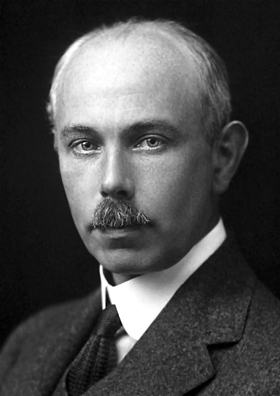
\includegraphics[width=\linewidth]{images/book3/aston.jpg}
\end{minipage}\hspace{0.02\linewidth}%
\begin{minipage}[t]{0.24\linewidth}
\vspace{0pt}
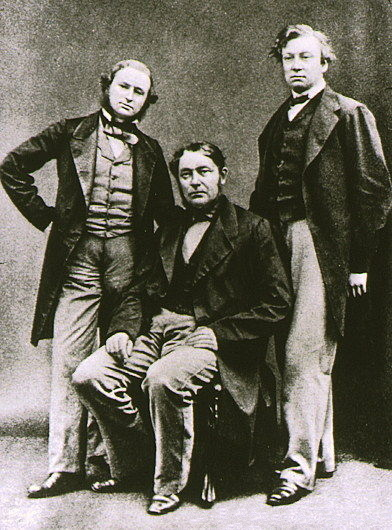
\includegraphics[width=\linewidth]{images/book3/kirchhoff-bunsen.jpg}
\end{minipage}\hfill
\begin{minipage}[t]{0.54\linewidth}
\vspace{0pt}
Gustav Kirchhoff and Robert Bunsen showed around 1860 that each element gives its own lines in a flame,
and discovered caesium and rubidium by their unknown lines. Francis Aston's mass spectrograph, from
1919, showed that most elements are mixtures of isotopes; he received the 1922 Nobel Prize in Chemistry.
(Photographs: Aston, unknown author, public domain; Kirchhoff, Bunsen and Henry Roscoe in 1862, from
Roscoe's collection, public domain; Wikimedia Commons.)
\end{minipage}
\end{history}

\section{Exercises}

\begin{exercise}[$\star$]\label{exo:b2:mass-spec-atomic:1}
Give the $m/z$ of: the \omterm{def:b2:mass-spec-atomic:molecular-ion}{molecular ion} of benzene \ce{C6H6}; an ion of mass \qty{400}{u} carrying two
charges; the protonated molecule of caffeine (\ce{C8H10N4O2}, nominal mass 194) formed by electrospray.
\end{exercise}

\begin{exercise}[$\star$]\label{exo:b2:mass-spec-atomic:2}
A compound of C, H, N and O has a \omterm{def:b2:mass-spec-atomic:molecular-ion}{molecular ion} at $m/z$ 73. What can be said of its nitrogen atoms?
Propose a formula.
\end{exercise}

\begin{exercise}[$\star$]\label{exo:b2:mass-spec-atomic:3}
A molecular-ion cluster shows two peaks two units apart, of nearly equal height. Another shows two
peaks two units apart in the ratio 3 : 1. Which halogens?
\end{exercise}

\begin{exercise}[$\star$]\label{exo:b2:mass-spec-atomic:4}
A salt colours a flame yellow; another crimson. Identify the elements and give the wavelengths of their
lines.
\end{exercise}

\begin{exercise}[$\star\star$]\label{exo:b2:mass-spec-atomic:5}
A hydrocarbon has $M$ at 100 \% and $M+1$ at 6.7 \%. How many carbon atoms does it contain?
\end{exercise}

\begin{exercise}[$\star\star$]\label{exo:b2:mass-spec-atomic:6}
Compute the exact masses of \ce{CO}, \ce{N2} and \ce{C2H4} and the resolving power needed to separate
each pair.
\end{exercise}

\begin{exercise}[$\star\star$]\label{exo:b2:mass-spec-atomic:7}
The EI spectrum of pentan-3-one shows peaks at 86, 57 (\omterm{def:b2:mass-spec-atomic:spectrum}{base peak}) and 29. Assign them.
\end{exercise}

\begin{exercise}[$\star\star$]\label{exo:b2:mass-spec-atomic:8}
The spectrum of pentan-2-one shows peaks at 86, 71, 58 and 43 (\omterm{def:b2:mass-spec-atomic:spectrum}{base peak}). Assign them, and explain
why pentan-3-one shows no peak at 58.
\end{exercise}

\begin{exercise}[$\star\star$]\label{exo:b2:mass-spec-atomic:9}
Copper standards at 1.0, 2.0, 3.0 and \qty{4.0}{mg/L} give absorbances 0.052, 0.104, 0.155 and 0.207;
a sample gives 0.128 (exercise data). Compute its copper concentration.
\end{exercise}

\begin{exercise}[$\star\star\star$]\label{exo:b2:mass-spec-atomic:10}
In a time-of-flight analyser, $L = \qty{1.00}{m}$ and $U = \qty{20.0}{kV}$. Compute the flight time of
a singly charged ion of mass \qty{1000}{u}, and the time separating it from an ion of \qty{1001}{u}.
\end{exercise}

\begin{exercise}[$\star\star\star$]\label{exo:b2:mass-spec-atomic:11}
Compute the molecular-ion cluster of dichloromethane, \ce{CH2Cl2}: $m/z$ values and relative
intensities.
\end{exercise}

\begin{exercise}[$\star\star\star$]\label{exo:b2:mass-spec-atomic:12}
In ICP-MS, \ce{^{40}Ar^{16}O+} interferes with \ce{^{56}Fe+}. Compute the resolving power needed to
separate them, and propose another way out.
\end{exercise}

\section{Problem: An Unknown Halide}

\begin{problem}[{Weekend problem --- a molecular-ion cluster with chlorine and bromine, the number of
carbons, the fragments, and a structure checked against every peak}]
\label{pb:b2:mass-spec-atomic:1}
A colourless liquid, eluted as one peak by \omterm{def:b2:chromatography:techniques}{gas chromatography}, gives the EI \omterm{def:b2:mass-spec-atomic:spectrum}{mass spectrum} below (NIST
WebBook data). Main peaks ($m/z$: relative intensity): 156: 14.5; 157: 0.5; 158: 18.6; 159: 0.6; 160:
4.4; 107: 6.7; 109: 6.3; 93: 3.3; 95: 2.9; 77: 59; 79: 18.7; 76: 39.5; 49: 12.9; 51: 4.3; 41: 100; 39:
26.2; 27: 24.6. Isotopic abundances: \ce{^{35}Cl} 0.758, \ce{^{37}Cl} 0.242, \ce{^{79}Br} 0.5069,
\ce{^{81}Br} 0.4931, \ce{^{12}C} 0.989, \ce{^{13}C} 0.011.
% ledger: ms:bromochloropropane, iso:Cl35, iso:Cl37, iso:Br79, iso:Br81, iso:C12, iso:C13, mass:C12, mass:H1, mass:Br79, mass:Cl35

\begin{center}
\begin{tikzpicture}
\begin{axis}[width=0.8\linewidth, height=4.6cm, xmin=20, xmax=170, ymin=0, ymax=112,
  xlabel={$m/z$}, ylabel={relative intensity}, label style={font=\small},
  tick label style={font=\scriptsize}, ycomb, xtick={27,41,49,77,93,107,122,156}]
\addplot[omDef, thick] table[x=mz, y=I] {figdata/out/bachelor-2-mass-spectra-d.dat};
\end{axis}
\end{tikzpicture}
\end{center}
% figdata: bachelor-2/mass-spectra.py part d

\medskip
\noindent\textbf{Part I --- The \omterm{def:b2:mass-spec-atomic:molecular-ion}{molecular ion}.}
\begin{enumerate}
  \item Which peaks form the molecular-ion cluster? Why is it not a single peak?
  \item Which halogens does a three-peak cluster spaced by 2 suggest?
  \item What is the nominal mass of the lightest isotopic form?
  \item What does the \omterm{def:b2:mass-spec-atomic:nitrogen-rule}{nitrogen rule} say?
  \item Subtract one \ce{^{79}Br} and one \ce{^{35}Cl}: what remains, and which hydrocarbon fragment
        has that mass?
  \item Propose a molecular formula and give its degree of unsaturation.
\end{enumerate}

\medskip
\noindent\textbf{Part II --- Carbons and exact mass.}
\begin{enumerate}[resume]
  \item From the 157/156 ratio, estimate the number of carbons.
  \item Why is that estimate rough here?
  \item Which isotopic forms contribute to the peak at 158?
  \item Compute the \omterm{def:b2:mass-spec-atomic:exact-mass}{monoisotopic mass} of the \omterm{def:b2:mass-spec-atomic:molecular-ion}{molecular ion}.
  \item \ce{C10H20O} also has nominal mass 156 (exact 156.151). What resolving power separates the
        two?
  \item Would the \omterm{def:b2:mass-spec-atomic:molecular-ion}{molecular ion} of a compound with a C=C bond and the same halogens have a different
        nominal mass?
\end{enumerate}

\medskip
\noindent\textbf{Part III --- Fragments.}
\begin{enumerate}[resume]
  \item The pair 77/79 is in the ratio 3 : 1. Which atom has been lost, and what is the ion?
  \item Explain the peak at 76.
  \item Assign the \omterm{def:b2:mass-spec-atomic:spectrum}{base peak} at 41.
  \item Assign the pair 49/51.
  \item Assign the pairs 93/95 and 107/109.
  \item Why is a bromine atom lost more easily than a chlorine atom?
  \item 1-Bromo-1-chloropropane would give \ce{CHBrCl+} at 127, 129 and 131. Does the spectrum support
        it?
\end{enumerate}

\medskip
\noindent\textbf{Part IV --- The structure.}
\begin{enumerate}[resume]
  \item Propose the structure.
  \item Check that it explains each peak listed.
  \item Can a \omterm{def:b2:mass-spec-atomic:fragmentation}{McLafferty rearrangement} occur? Why?
  \item Draw the isomer that would give a strong peak at $m/z$ 63/65 and none at 49/51.
  \item Which isotopic forms make the peak at 160?
  \item From the isotopic abundances, compute the ratio of the $M$, $M+2$ and $M+4$ peaks for one
        chlorine and one bromine, and compare it with the spectrum.
\end{enumerate}
\end{problem}
